\chapter{Keamanan Sistem Email}

{\em Electronic mail} (email\footnote{Dalam bahasa Indonesia sudah ada istilah
{\bf surel} untuk email ini. Dalam buku ini saya masih menggunakan istilah
email.}) masih merupakan salah satu aplikasi yang paling populer di internet.
Bahkan alamat email digunakan sebagai identitas pengguna di internet. Jika Anda
mendaftar ke sebuah layanan, email digunakan sebagai identitas.

Beberapa masalah keamanan terkait dengan sistem email antara lain:
\begin{itemize}
\item disadap ({\em intercept});
\item dipalsukan ({\em forgery});
\item disusupi ({\em intrude});
\item digunakan untuk spamming;
\item mailbomb;
\item mail relay.
\end{itemize}

\section{Komponen Sistem Email}
Sebelum membahas masalah keamanan tersebut ada baiknya kita melihat komponen
dari sebuah sistem mail.
Sebuah sistem email terdiri dari beberapa komponen;
{\em mail user agent} (MUA),
{\em mail transfer agent} (MTA), dan
{\em mail delivery agent} (MDA).
(Lihat Gambar~\ref{fig:email-topologi}.)

\begin{figure}[ht]
\fbox{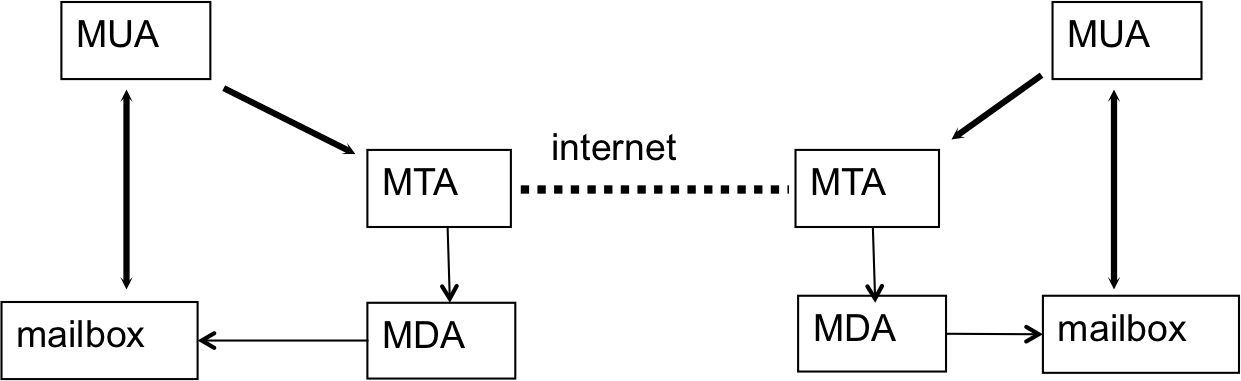
\includegraphics[width=1.0\linewidth]{graphics/email-topologi.png}}
\caption{Topologi Sistem Email}
\label{fig:email-topologi}
\end{figure}

MUA adalah komponen yang berhubungan dengan pengguna. Biasanya MUA adalah yang
kita sebut program email. Contoh dari MUA antara lain adalah Thunderbird,
Outlook, Mac Mail.app, mutt, UNIX mail, pine, dan masih banyak lagi. (Daftar
ini sering berubah.)
Pengguna menggunakan MUA untuk membuat ({\em compose}) dan membaca email.

MTA adalah komponen yang bertugas untuk mengirimkan dan menerima email. Dia
adalah ``pak pos''. MTA menerima berkas email dari MUA dan meneruskannya ke MTA
lainnya dan seterusnya sampai ke MTA yang dituju. Contoh dari MTA antara lain
adalah postfix, sendmail, qmail, Exchange, exim, dan sejenisnya. MTA biasanya
adalah urusan dari administrator.

MDA adalah komponen yang bertugas untuk menyimpan email yang datang ke mailbox
pengguna. Dahulu, MDA ini menjadi bagian dari MTA, tetapi kemudian dipisahkan
karena pemisahan role agar lebih aman. MDA harus menambahkan email yang baru
masuk ke mailbox pengguna. Untuk itu MDA harus memiliki hak untuk menulis ke
mailbox tersebut, dengan kata lain MDA harus dijalankan dengan hak admin atau
{\em super user / root}. Sementara itu MTA tidak harus dijalanakan sebagai admin.

Skenario yang terjadi adalah sebagai berikut. Seorang pengguna (A) membuat
email dengan menggunakan MUA. Setelah email selesai dibuat, email diberikan
kepada MTA untuk disampaikan kepada MTA penerima (B). Kadang MTA yang dituju
tidak langsung dapat diakses tetapi melalui MTA lainnya dahulu.  Sesampainya di
MTA tujuan, email diberikan ke MDA untuk ditambahkan ke mailbox penerima (B).
Penerima (B) tidak harus online ketika email tersebut itu sampai. Ketika
penerima (B) akan membaca email, maka dia akan menggunakan MUA untuk mengakses
mailbox. Jika dia (B) akan membalas, maka digunakan MUA untuk menuliskan
balasannya. Setelah selesai, email balasan diteruskan ke MTA untuk disampaikan
ke MTA tujuan (A).


\section{Standar Email}
Pengguna email memiliki sistem dan konfigurasi yang bervariasi. Masalah
{\em interoprability} merupakan salah satu aspek yang sangat penting. Untuk itu
digunakan RFC (Request For Comments) sebagai standar.

Standar format email didefinisikan oleh RFC 822, ``Standard for the format of 
ARPA Internet text messages.'' (RFC ini sudah digantikan oleh RFC~2822,
``Internet Message Format.'') Pada prinsipnya email dibagi dua bagian; {\bf
header} dan {\bf body}.

\begin{itemize}
   \item {\em Header}. Seperti amplop, berisi informasi tentang alamat pengirim
      yang dituju. Header ini berisi {\em field} yang nantinya digunakan oleh
      MTA untuk mengirimkan ke tujuan.
   \item {\em Body}. Isi surat. Body dipisahkan dari header dengan satu baris
      kosong. 
\end{itemize}

Contoh dari (format) email dapat dilihat sebagai berikut. Perhatikan bahwa
header dan body dipisahkan oleh satu baris kosong. Contoh ini tentu saja
merupakan simplifikasi dari format email sesungguhnya.

\begin{mdframed}
\begin{verbatim}
From: Budi Rahardjo <budi@cert.or.id>
To: br@paume.itb.ac.id
Subject: Kelas EL776 hari ini

Kelas hari ini dibatalkan dan akan digantikan dengan
hari lain.

-- budi
\end{verbatim}
\end{mdframed}

Ada standar {\em field} di header yang mudah terlihat oleh pengguna, yaitu {\em
From}, {\em To}, {\em Subject}. Padahal ada banyak {\em field-field} lain yang
biasanya terdapat dalam email. Berikut ini contoh header yang lebih komplit
lagi.

\begin{mdframed}
\begin{verbatim}
Received: from nic.cafax.se (nic.cafax.se [192.71.228.17])
   by alliance.globalnetlink.com (8.9.1/8.9.1) with ESMTP id QAA31830
   for <budi@alliance.globalnetlink.com>; Mon, 26 Mar 2001 16:18:01 -0600
Received: from localhost (localhost [[UNIX: localhost]])
	by nic.cafax.se (8.12.0.Beta6/8.12.0.Beta5) id f2QLSJVM018917
	for ietf-provreg-outgoing; Mon, 26 Mar 2001 23:28:19 +0200 (MEST)
Received: from is1-55.antd.nist.gov (is1-50.antd.nist.gov [129.6.50.251])
	by nic.cafax.se (8.12.0.Beta5/8.12.0.Beta5) with ESMTP id f2QLSGiM018912
	for <ietf-provreg@cafax.se>; Mon, 26 Mar 2001 23:28:17 +0200 (MEST)
Received: from barnacle (barnacle.antd.nist.gov [129.6.55.185])
	by is1-55.antd.nist.gov (8.9.3/8.9.3) with SMTP id QAA07174
	for <ietf-provreg@cafax.se>; Mon, 26 Mar 2001 16:28:14 -0500 (EST)
Message-ID: <04f901c0b63b$16570020$b9370681@antd.nist.gov>
From: "Scott Rose" <scottr@antd.nist.gov>
To: <ietf-provreg@cafax.se>
Subject: confidentiality and transfers
Date: Mon, 26 Mar 2001 16:24:05 -0500
MIME-Version: 1.0
X-Mailer: Microsoft Outlook Express 5.50.4133.2400
Sender: owner-ietf-provreg@cafax.se
Precedence: bulk
\end{verbatim}
\end{mdframed}
